\capitulo{5}{Aspectos relevantes del desarrollo del proyecto}\label{aspectos relevantes}

En este apartado se presentarán los aspectos relevantes del desarrollo del proyecto, exponiendo los problemas y las principales decisiones tomadas en cada una de las fases. Se distinguirá, de nuevo, entre la fase de investigación y la fase de desarrollo de la aplicación de Android. 

\section{Fase de investigación}

A continuación se expondrán las distintas situaciones que obligaron a tomar decisiones sobre cómo proseguir con la investigación y se explicará la razón por la que se tomó cada decisión concreta. También se hablará de detalles de implementación que fueron necesarios para abordar algunos de esos problemas. 

Cabe destacar que la fase de investigación se hizo de forma conjunta con mi compañero de proyecto José Luis Garrido Labrador, y que las decisiones se tomaron entre los dos y con la ayuda de nuestros tutores. 

\subsection{Exploración del estado del arte}

Como en cualquier proyecto de investigación, el paso inicial consistió en realizar una exploración del estado del arte sobre métodos y técnicas empleados para la detección automática de ataque epilépticos o de otros problemas similares, como la detección de caídas. En esta exploración se encontró que, aunque la detección automática de ataques epilépticos es un campo muy explorado, la mayoría de las técnicas que se encuentran se basan en el uso de Electroencefalogramas (EEG) y pulseras inteligentes basadas en la monitorización de las constantes vitales. Por otro lado, no se encontraron artículos relativos a técnicas o metodologías de aprendizaje a partir de los datos de sensores de presión instalados en colchones o similares.

Por otro lado, dado que el conjunto de datos disponibles es claramente desequilibrado (se tienen muchas más instancias de <<no crisis>> que de <<crisis>>) también se realizó una búsqueda de técnicas aplicadas a este tipo de problemas, lo que nos llevó a los modelos de clasificación expuestos en el apartado~\ref{conceptos teoricos} (Conceptos teóricos). 

\subsection{Etiquetado de los datos}

Uno de los principales problemas que se tuvo que afrontar fue el del etiquetado de los datos. Aunque los proveedores de los datos indicaron también un rango de horas en los que supuestamente tuvo lugar una crisis epiléptica, estos rangos eran muy aproximados y demasiado amplios para lo que dura una crisis epiléptica, según la bibliografía, sin que se produzcan consecuencias fatales o irreversibles~\cite{epilepsia}. 

Esto nos obligó a realizar una inspección visual de los datos, y ajustar los tiempos de la crisis teniendo en cuenta: 

\begin{itemize}
	\item Los rangos de horas proporcionados por los proveedores de los datos. 
	\item Información relativa al aspecto de las señales en entornos próximos al inicio y final de esos rangos. 
	\item Información relativa a las proyecciones obtenidas mediante las técnicas de reducción de la dimensionalidad, de forma que, si existía algún tipo de separación, se aplicaron las etiquetas de <<crisis>> a solamente aquellas instancias dentro de los rangos que mostraban una separación más clara con las instancias de <<no crisis>>. 
\end{itemize}

\begin{figure}
	\centering
	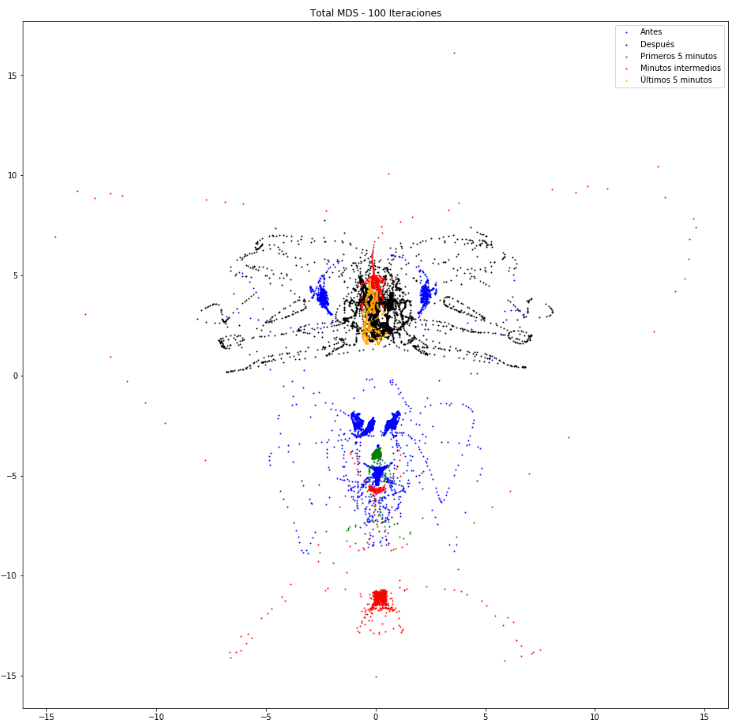
\includegraphics[width=0.7\textwidth]{../img/mdsetiquetado.png}
	\caption{Aplicación de \textit{MDS} para el etiquetado de la primera crisis.}
	\label{fig:mdsetiquetado}
\end{figure}

En la figura~\ref{fig:mdsetiquetado} se muestra la aplicación de la técnica de transformación MDS para el etiquetado de la primera crisis. Las instancias se han dividido en colores en función de su instante de tiempo respecto al rango proporcionado por los proveedores de los datos. (Azul: antes de la crisis, Negro: después de la crisis, Verde: primeros 5 minutos de la crisis, Rojo: minutos centrales de la crisis, Naranja: últimos 5 minutos de la crisis). Como se puede observar, las instancias rojas presentan una separación mucho mayor con el resto, y además coinciden con aquellas cuyas señales de presión mostraban una diferencia más significativa dentro de su entorno, por lo que esas fueron las instancias etiquetadas como <<crisis>>. 

Se debe tener en cuenta que, aunque se realizaron estos ajustes, el etiquetado de los datos no puede ser considerado otra cosa que aproximado, y se asume que por esta razón los datos tendrán cierto grado de ruido. Este motivo junto con la escasez de datos de <<crisis>> en el conjunto de datos disponible, representan los mayores problemas a los que me he tenido que enfrentar en el proyecto. 

\subsection{Limpieza de datos}

Del total de datos, hubo que desechar muchas de las instancias por distintas razones. En primer lugar se eliminaron aquellas instancias cuya señal era de mala calidad. Concretamente eliminamos todas aquellas instancias con un SS menor de 400 (como recomendaban los proveedores de los datos), pero no tuvimos en cuenta el valor de STATUS ya que, como se explicará más adelante, los valores de las constantes vitales no se usaron para la búsqueda del modelo de clasificación.

Por otra parte, mediante una inspección inicial de los datos se detectó que algunos datos de los tubos de presión en ocasiones eran negativos (lo cual no debería ocurrir), y aparecían valores bajos de presión en momentos en los que la cama debería estar vacía. Por esta razón, se decidió considerar todo valor de presión menor a 5 como ruido convirtiéndolo automáticamente a 0. De esta forma nos deshicimos también de los valores negativos. Para eliminar el ruido del resto de los datos se aplicó un filtro de Butterworth.

En esta inspección también se advirtió que los atributos referentes a las constantes vitales eran nulos de forma intermitente y en una gran cantidad de las instancias. Como supimos más adelante, esto se debió al mal funcionamiento del sensor durante las primeras etapas de recogida de los datos. Aunque algunas técnicas de minería de datos soportan la presencia de atributos desconocidos (\textit{missing}) en algunas de las instancias, la cantidad de instancias con constantes vitales nulas o incorrectas era tan grande que se tomó la decisión de no tener en cuenta estos datos para el resto de experimentos. Cabe destacar que esto supone un gran inconveniente, ya que la mayoría de técnicas de detección automática encontrados en el estado del arte (quitando las centradas en EEG) se basan en datos biométricos. 

\subsection{Selección de atributos}

A continuación se detectaron los atributos con baja variabilidad para su eliminación. Tras llevar a cabo este proceso se eliminaron los atributos P7, P8, P9, P10, P11 y P12. Esto tiene sentido ya que esos campos corresponden con la matriz de tubos de presión de una de las mitades del modelo de colchón de matrimonio, y el colchón con el que se trabaja en este proyecto es individual. Por esta razón eliminar estos datos no supone ninguna pérdida de información y, además, reduce a la mitad la cantidad de datos con la que deben tratar los modelos, lo que repercute positivamente en los tiempos. 

\subsection{Transformadores}

Una vez seleccionado el abanico de operaciones que íbamos a tener en cuenta para la búsqueda de un preprocesado óptimo, se codificaron estas operaciones como transformadores compatibles con sklearn para poder aplicarlas de forma sencilla y sistemática. Para ello se generaron una serie de clases que heredaban de la clase \texttt{sklearn.base.TransformerMixin}. En total se codificaron 9 transformadores. 


\subsection{Elección del tamaño de ventana}

Como se ha comentado en el apartado~\ref{conceptos teoricos} de Conceptos teóricos, para calcular estadísticas móviles del conjunto de datos debemos escoger un tamaño de ventana. Para determinar el valor óptimo para este problema, se realizó un barrido de tamaños aplicados a la media y la desviación móviles, datos que se usaron para entrenar y evaluar un clasificador \textit{Random Forest}. El proceso que se siguió se explica también con detenimiento y detalle en el apéndice del cuaderno de investigación. 

Para calcular las estadísticas móviles durante la exploración se usó nuestro transformador \texttt{StatisticsTransformer} que utiliza internamente las funciones  \texttt{df.rolling(window\_length).mean()} o \texttt{.std()} según el caso, donde \texttt{df} es el \texttt{pandas.DataFrame} que contiene los datos originales. Esta función devuelve un nuevo \texttt{pandas.DataFrame} con las estadísticas móviles calculadas para cada una de las ventanas (una fila por cada desplazamiento de la ventana). De esta forma, nos evita ir desplazando la ventana manualmente mediante un bucle. 

\begin{figure}[H]
	\centering
	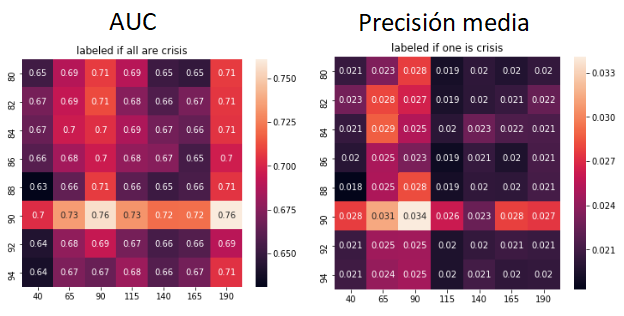
\includegraphics[width=1\textwidth]{../img/heatmap.png}
	\caption[Mapa de calor de los resultados finales de la exploración para cada uno de las métricas de evaluación.]{Mapa de calor de los resultados finales de la exploración para cada uno de las métricas de evaluación. En el eje $y$ el tamaño de la ventana para la desviación típica, en el eje $x$ el tamaño para la media.}
	\label{fig:heatmap}
\end{figure}

Para cada una de las métricas de evaluación del clasificador (AUC y Precisión media) se hicieron una serie de barridos de parámetros, centrándose cada vez más en los rangos en los que se lograba un mejor rendimiento, y llegando finalmente a los resultados que se muestran en la figura~\ref{fig:heatmap}. Como se puede observar, los mejores valores se lograron para un tamaño de ventana de 90 instancias, tanto para la desviación típica como para la media, y también para ambas métricas de evaluación. Por esta razón se usó este valor en los experimentos y también como tamaño de ventana para la extracción de características de series temporales. 

\subsection{Extracción de características de series temporales para una ventana de datos}

La extracción de características de series temporales aplicada a un cierto tamaño de ventana no es tan sencilla y merece un comentario sobre cómo se ha resuelto. La función encargada de la extracción de características pertenece a la biblioteca \texttt{tsfresh} y se llama \texttt{extract\_features}. Esta función recibe un \texttt{pandas.DataFrame} como parámetro y devuelve una fila de características por cada grupo de filas con el mismo <<id>> (debemos añadir un atributo <<id>> a nuestro conjunto de datos en bruto). Puedes indicarle mediante un diccionario pasado como parámetro el conjunto de características concreto que se desea calcular o, por el contrario, hacer que calcule todo su repertorio de características. Esta misma biblioteca ofrece una función llamada \texttt{utilities.dataframe\_functions.roll\_time\_series()} que, a efectos prácticos, permite la extracción de características aplicada a una ventana, pero lo hace con un coste de memoria tan grande que no resulta práctica para conjuntos de datos como el nuestro. Básicamente, crea un \texttt{pandas.DataFrame} con un <<id>> distinto para cada ventana. Pongamos un ejemplo para comprender su funcionamiento: si tenemos un conjunto de datos con 10 filas y queremos aplicar una ventana de tamaño 3, esta función devuelve: 
\begin{itemize}
	\item 3 filas correspondientes a las filas 1, 2, y 3 del conjunto original y con un <<id>>=1. 
	\item 3 filas correspondientes a las filas 2, 3, y 4 del conjunto original y con un <<id>>=2. 
	\item así sucesivamente. 
\end{itemize}

\begin{figure}[H]
	\centering
	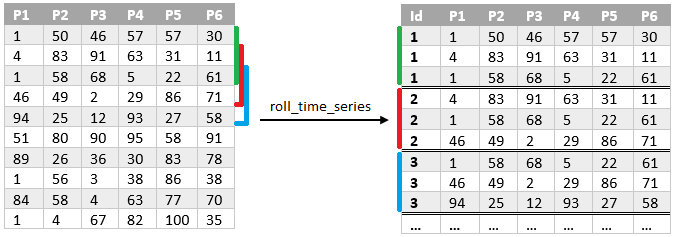
\includegraphics[width=1\textwidth]{../img/rolltimeseries.png}
	\caption{Ejemplo del funcionamiento de la función \texttt{roll\_time\_series}}
	\label{fig:rolltimeseries}
\end{figure}

Por cómo funciona en relación al atributo <<id>>, si aplicamos este nuevo conjunto de datos a la función \texttt{extract\_features} obtenemos lo que buscamos: una fila de características por cada ventana, pero el coste computacional y de memoria que supone la generación de este nuevo conjunto, que tiene una enorme cantidad de datos repetidos, es tan alto que no resulta viable. Por ello, en lugar de usar esta función, se tomó la decisión de realizar el desplazamiento de la ventana de forma manual mediante un bucle.


\subsection{Filtrado de características de series temporales}

Al ejecutar la extracción de características de las datos de las dos noches en las que tuvo lugar una crisis epiléptica, obtenemos 4\,764 características en total, 794 por cada tubo de presión. Este número de atributos es excesivo para aplicarlo directamente a un clasificador, por lo que planteamos varias estrategias para quedarnos con aquellos que aporten mayor información. Estas estrategias se encuentran recogidas y explicadas en el Anexo del Cuaderno de investigación, por lo que aquí se expone la que, por presentar un mejor rendimiento, se empleó como entrada a métodos de selección posteriores. 

Este filtrado consistió en usar la función \texttt{select\_features} de la biblioteca tsfresh, que realiza una selección supervisada de las características (recibe el el valor de las etiquetas de cada instancia). Al aplicar esta función el número de características se redujo a 1\,731. Además, asumimos que una característica solo sería relevante si resulta relevante para todos los tubos de presión, por lo que eliminamos aquellas que, tras el filtrado, no permanecieran para todos los tubos, quedándonos únicamente con 744 (124 para cada tubo de presión).  

\subsection{Selección final de características mediante algoritmo genético}

Una vez obtenidas las características más relevantes, es decir, que aportan más información, el último paso consiste en seleccionar un subconjunto más pequeño de ellas que sea suficiente para lograr un buen rendimiento del clasificador. De nuevo, se plantearon varias estrategias cuyo desarrollo se puede consultar en el cuaderno de investigación, y aquí se expondrá la que obtuvo un mejor rendimiento. 

Esta estrategia es la que emplea un algoritmo genético implementado mediante la biblioteca DEAP. Una de las decisiones que hay que tomar a la hora de diseñar un algoritmo genético es qué tipo de genotipo se va a utilizar. En este caso se decidió que el genotipo sería un array unidimensional en el que cada gen (cada posición del array) contiene un número entero entre 0 y 123, que hace referencia a cada una de las 124 características resultantes del filtrado. El tamaño de este array corresponderá con el tamaño máximo de características que pueden ser seleccionadas, y se tomó la decisión de restringir este valor a únicamente 10 características, para que fuera cual fuera el tipo de clasificador escogido finalmente, la clasificación fuese rápida. Esto es importante ya que, en teoría, debe aplicarse a un sistema de recepción de datos en tiempo real. 

\begin{figure}[H]
	\centering
	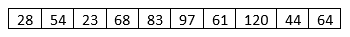
\includegraphics[width=0.7\textwidth]{../img/genotipo.png}
	\caption{Genotipo del mejor individuo encontrado usando el AUC como métrica de evaluación.}
	\label{fig:genotipo}
\end{figure}

Se aclara que 10 es el tamaño \textbf{máximo} de características porque, debido a los mecanismos de mutación y cruce utilizados, una característica puede aparecer más de una vez en un mismo individuo, en cuyo caso solo se tendría en cuenta una vez. Esta decisión se tomó porque de los mecanismos de cruce y mutación que ofrece DEAP, ninguno está preparado para trabajar con pseudopermutaciones (permutaciones en las que el tamaño del array no corresponde con el número de valores que puede contener). Aunque en DEAP es posible crear mecanismos de cruce y mutación personalizados que resolverían este problema, el beneficio que se obtiene con ello es mínimo o nulo. Esto se debe a que al tratar de maximizar el rendimiento, prevalecerán aquellos individuos que aporten mayor información al clasificar, es decir, aquellos con un mayor número de características.

Esto nos lleva a la decisión de cómo implementar la función de adaptación. Como ya hemos comentado, tenemos características relativas a dos noches en las que tuvo lugar una crisis epiléptica, y queremos realizar una evaluación lo más dura posible para que estemos seguros de que el clasificador vaya a predecir bien nuevas instancias. Por esta razón decidimos que la evaluación de los individuos se realizará mediante validación cruzada entre dos días (este tipo de evaluación se usó a menudo en otras fases de la investigación): 

\begin{minipage}{\linewidth}
\begin{enumerate}
	\item Se entrena un clasificador \textit{Random Forest} con las características indicadas por el genotipo del individuo, pero solo con los datos pertenecientes a la noche de la primera crisis. 
	\item Se calcula el rendimiento del clasificador de acuerdo a la métrica pertinente (se usó tanto el AUC como la Precisión media) tomando los datos pertenecientes a la noche de la segunda crisis como partición de test. 
	\item Se realiza el proceso inverso. 
	\item La función de adaptación devolverá la media de los dos rendimientos obtenidos, el cual se tratará de maximizar. 
\end{enumerate}
\end{minipage}

Las últimas decisiones que se deben tomar en relación a la configuración del algoritmo son el tamaño de la población y el número de generaciones que se ejecutan. En ambos casos se escoge un valor de 50 teniendo en cuenta lo costosa que es la evaluación de cada individuo, y se confirma la decisión al ver que tras la ejecución se observa que no se producen mejoras en las últimas generaciones. 

\begin{figure}
	\centering
	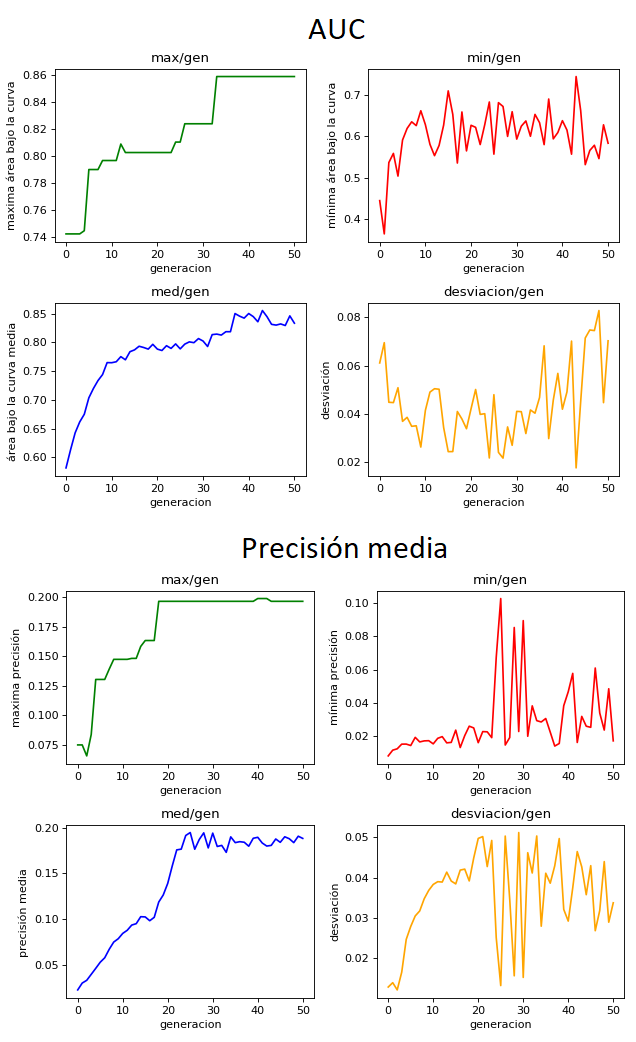
\includegraphics[width=0.8\textwidth]{../img/genetico.png}
	\caption{Evolución del algoritmo genético para cada una de las métricas de evaluación consideradas.}
	\label{fig:genetico}
\end{figure}

\subsection{One-Class y \textit{ensembles} para desequilibrados}

Las características seleccionadas mediante el algoritmo genético no se probaron unicamente en un clasificador \textit{Random Forest}, sirvieron como entrada para otros tipos de clasificador, como los comentados en el apartado~\ref{conceptos teoricos} de Conceptos teóricos. Sin embargo, fue mi compañero José Luis Garrido Labrador el que se centró más en esta parte de la investigación, por lo que los aspectos relevantes relativos a estos clasificadores, así como a la detección de anomalías One-Class, se recogerán en su memoria. 

En resumen, aquí se pueden exponer los resultados conseguidos al utilizar, como datos de entrenamiento, el conjunto de características seleccionado por el algoritmo genético usando la métrica de la precisión media en la función de adaptación, ya que, según la bibliografía~\cite{Davis2006RPR, saito2015pr}, esta métrica es más adecuada para la evaluación de clasificadores en conjuntos de datos desequilibrados. 

Como se explica en el apéndice del cuaderno de investigación, tras una exploración más amplia de varios tipos de clasificador, finalmente se escogen y comparan 3 métodos de remuestreo junto con 3 tipos de \textit{ensembles} distintos. Los métodos de remuestreo son: \textit{Random Balance} (RB)~\cite{diez2015random}, \textit{SMOTE} (SM)~\cite{galar2012review} y \textit{Random under sampling} (RUS)~\cite{diez2015diversity}. Los \textit{ensembles} son: \textit{Bagging} (Bag)~\cite{galar2012review}, \textit{Rotation Forest} (RotF)~\cite{rodriguez2006rotation} y \textit{RandomCommittee} (RC)~\cite{diez2015diversity}. Las tablas~\ref{tab:crisis1} y~\ref{tab:crisis2} muestran los resultado medios obtenidos para 10 ejecuciones con cada una de las combinaciones de remuestreo-\textit{ensemble}. Cada fila corresponde con un método distinto y cada columna con una métrica de rendimiento, donde \textit{TPR}=tasa de verdaderos positivos, \textit{FPR}=tasa de falsos positivos, \textit{TNR}=tasa de verdaderos negativos, \textit{FNR}=tasa de falsos negativos, \textit{PRC}=\textit{Precision-Recall} (precisión media), \textit{ACC}=área bajo la curva ROC y \textit{ACC}=\textit{accuracy}. 

\begin{table}\scriptsize
	\begin{center}
		\begin{tabular}{llllllll}
			\toprule
			{}Algoritmo & TPR &          FPR &       TNR & FNR &       PRC &       AUC &       ACC \\
			\midrule
			RB - Bag                &   0 &            0 &         1 &   1 &  0.984425 &  0.552363 &   0.98178 \\
			RB - RC       &   0 &            0 &         1 &   1 &  0.981267 &  0.485675 &   0.98178 \\
			RB - RotF        &   0 &  1.65036e-06 &  0.999998 &   1 &  0.980551 &  0.485354 &  0.981778 \\
			RUS - Bag          &   0 &  0.000899444 &  0.999101 &   1 &  0.980613 &  0.447139 &  0.980897 \\
			RUS - RC &   0 &            0 &         1 &   1 &  0.981076 &    0.4806 &   0.98178 \\
			RUS - RotF  &   0 &  0.000394435 &  0.999606 &   1 &  0.982287 &  0.486412 &  0.981393 \\
			SM - Bag                         &   0 &  0.000173287 &  0.999827 &   1 &  0.984367 &  0.565807 &   0.98161 \\
			SM - RC                &   0 &            0 &         1 &   1 &  0.981278 &  0.486071 &   0.98178 \\
			SM - RotF                 &   0 &  1.56784e-05 &  0.999984 &   1 &  0.982673 &  0.512364 &  0.981764 \\
			\bottomrule
		\end{tabular}
		\caption{Resultados para el entrenamiento con la primera crisis y testeo con la segunda crisis.}
		\label{tab:crisis1}
	\end{center}
\end{table}

\begin{table}\scriptsize
	\begin{center}
		\begin{tabular}{llllllll}
			\toprule
			{}Algoritmo & TPR &         FPR &       TNR & FNR &       PCR &       AUC &       ACC \\
			\midrule
			RB - Bag                &   0 &   0.0109634 &  0.989037 &   1 &  0.995225 &  0.491511 &  0.983616 \\
			RB - RC       &   0 &  0.00571683 &  0.994283 &   1 &  0.993912 &  0.446135 &  0.988834 \\
			RB - RotF        &   0 &  0.00488364 &  0.995116 &   1 &   0.99517 &  0.525534 &  0.989663 \\
			RUS - Bag          &   0 &   0.0461306 &  0.953869 &   1 &  0.994863 &  0.514533 &  0.948642 \\
			RUS - RC &   0 &   0.0112769 &  0.988723 &   1 &  0.994602 &  0.506568 &  0.983304 \\
			RUS - RotF  &   0 &   0.0128567 &  0.987143 &   1 &  0.994482 &  0.468075 &  0.981733 \\
			SM - Bag                         &   0 &    0.017596 &  0.982404 &   1 &  0.995505 &  0.539099 &   0.97702 \\
			SM - RC                &   0 &   0.0048424 &  0.995158 &   1 &  0.994052 &  0.458383 &  0.989704 \\
			SM - RotF                 &   0 &  0.00344412 &  0.996556 &   1 &  0.994742 &  0.502318 &  0.991094 \\
			\bottomrule
		\end{tabular}
		\caption{Resultados para el entrenamiento con la segunda crisis y testeo con la primera crisis.}
		\label{tab:crisis2}
	\end{center}
\end{table}

\subsection{Ejecución remota de experimentos con \textit{tmux}}

Como ya se ha explicado al hablar de tmux en el apartado \ref{tecnicas y herramientas} (Técnicas y herramientas), nos hemos topado con un problema al tratar de ejecutar experimentos computacionalmente costosos en el equipo de cómputo del grupo de investigación de los tutores. 

Normalmente, para lanzar los experimentos en el equipo, nos hemos conectado mediante ssh, y hemos lanzado el proceso de jupyter notebook sin interfaz gráfica mediante el comando \texttt{jupyter notebook ---no-browser}. Este comando devuelve una URL que podemos copiar en nuestro navegador local para acceder a la interfaz gráfica del proceso y ejecutar los experimentos. Para ejecutar notebooks sin necesidad de acceder a la interfaz gráfica se ha usado el comando \texttt{jupyter nbconvert}. 

Sin embargo, mediante este proceso, para experimentos muy costosos la conexión ssh se cerraba en mitad del trabajo y se perdían los resultados. Por ello, hemos usado el multiplexador de terminales tmux, que permite iniciar varias sesiones y ejecutarlas en segundo plano. De esta forma aunque se pierda la conexión ssh, un proceso lanzado en una de esas sesiones seguirá corriendo en el equipo, y podremos acceder a los resultados recuperando la conexión una vez termine. 

\section{Fase de desarrollo de la aplicación}

A continuación se expondrán los problemas y las decisiones que se tomaron referentes al desarrollo de la aplicación de Android. A diferencia de la fase de investigación, la fase de desarrollo se llevó a cabo de forma individual, pero debido a que la lógica de negocio se basó en la comunicación con la API desarrollada por mi compañero, algunas de las decisiones estuvieron condicionadas por las suyas. 

\subsection{Formación en Android}

El desarrollo de una aplicación en Android requiere de unos conocimientos previos de los que no disponía antes de comenzar este proyecto, por lo que el primer paso consistió en buscar recursos que me permitieran iniciarme en el tema de la forma más eficiente posible. Estos recursos fueron principalmente los siguientes: 

\begin{itemize}
	\item El curso online gratuíto \textit{Android Development for Beginners} de Google (Udacity)~\cite{udacity}, que se estructura en los siguientes temas: 
	
	\begin{minipage}{\linewidth}
	\begin{itemize}
		\item \textit{User input} (Aprox. 4 Semanas)
		\item \textit{Multiple App Screens} (Aprox. 2 meses)
		\item \textit{Networking} (Aprox. 5 semanas)
		\item \textit{Data Storage} (Aprox. 8 semanas)
	\end{itemize}
	\end{minipage}
	
	Este curso está preparado para personas sin ningún conocimiento de programación previo, por lo que los tiempos estimados son demasiado amplios para alguien que ya cuenta con conocimientos de programación en Java y diseño y desarrollo de software en general. 
	\item La página web de \textit{Android Developers}~\cite{androiddevelopers}, que contiene la documentación oficial de las herramientas del SDK de Android y la API. 
	\item La página web de \textit{Stack Overflow}~\cite{stackoverflow}, donde se encontró solución a muchas de las pequeñas cuestiones que surgieron a lo largo del desarrollo. 
\end{itemize}

El curso me permitió adquirir las bases necesarias para comenzar con el desarrollo de la aplicación, y en los demás recursos encontré solución a cuestiones de implementación más concretas. 

\subsection{Inicio del desarrollo}

Para empezar, una de las primeras decisiones que se tomó fue para qué versiones de Android se iba a desarrollar la aplicación. Tras consultar el porcentaje de usuarios de cada versión de Android en el momento~\cite{paneldecontrol}, se tomó la decisión de dar soporte a la versión 6.0 \textit{Marshmallow} (API 23) y superiores, cubriendo un 74,8\% de los dispositivos Android del mercado. Aunque la versión 5.1 contaba con un porcentaje relativamente importante de usuarios, del 11,5\%, la aplicación resultante no iba a ser puesta en producción de inmediato, por lo que se consideró que las versiones soportadas eran suficientes. 

\subsection{Resumen de la arquitectura de la aplicación}

La arquitectura puede verse desde dos puntos de vista distintos. Si consideramos el sistema como una entidad completa, incluyendo la aplicación cliente y la API del servidor, podemos hablar, como hace mi compañero en su memoria, de arquitectura Modelo-Vista-Controlador (MVC), dentro de la cual mi aplicación sería considerada como una Vista, ya que la lógica de negocio está enteramente contenida en la API. 

Por otro lado, si hablamos de aplicaciones que trabajan directamente con los datos proporcionados por una API encontramos menciones a lo que comúnmente se denomina <<arquitectura de microservicios>>. Según esta arquitectura, cada funcionalidad está contenida en un proceso del servidor, de forma que cada parte de la lógica de negocio se encuentra encapsulada y los procesos son independientes entre sí. El cliente se limita a hacer peticiones a los microservicios de la API del servidor para acceder a la lógica de negocio. 

\begin{figure}[H]
	\centering
	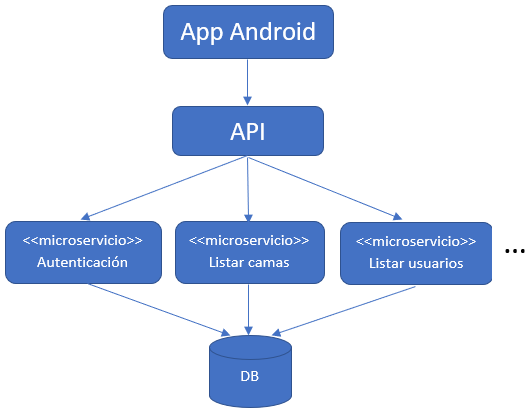
\includegraphics[width=0.8\textwidth]{../img/microservicios.png}
	\caption{Abstracción de la arquitectura de microservicios.}
	\label{fig:microservicios}
\end{figure}

\subsection{Comunicación con la API}

Como se expone detenidamente en el apéndice de Especificación de requisitos, la aplicación ofrecerá, a grandes rasgos, tres funcionalidades principales: 

\begin{enumerate}
	\item \textbf{Gestión de usuarios:} permite gestionar qué usuarios y con qué credenciales pueden acceder al sistema. Esta funcionalidad solo estará disponible para el usuario con rol de admnistrador. 
	\item \textbf{Gestión de camas:} permite gestionar las camas instaladas y qué usuarios tienen acceso a sus datos. También estará disponible solo para el usuario administrador. 
	\item \textbf{Visualización de camas:} permite visualizar en tiempo real los datos captados por las camas a las que el usuario tiene acceso. El usuario administrador tendrá acceso a todas las camas instaladas, el resto solo a las especificadas por el administrador. 
\end{enumerate}

Todas estas funcionalidades se basan en los servicios disponibles en la API de mi compañero. Las especificaciones de la API se exponen en el Manual del programador contenido en los anexos de su trabajo, donde se explica que se distingue entre dos tipos de comunicación: 

\begin{enumerate}
	\item La mayor parte de los servicios se basan en peticiones POST a rutas específicas en función del servicio. Este tipo de comunicación abarca servicios de autenticación, consulta y modificación de datos de gestión (tanto de usuarios como de camas). 
	\item De forma particular, el sistema que proporciona los datos captados por las camas en tiempo real se maneja a través de mensajes entre \textit{WebSockets} usando la librería Socket.IO. 
\end{enumerate}

\subsubsection{Peticiones POST}
Dado que el funcionamiento de la aplicación depende casi enteramente de la comunicación con la API, debemos estar seguros de que existe conexión antes de realizar cada petición POST. Además, tal y como se implementa la API, un usuario solo puede mantener la autenticación en un dispositivo al mismo tiempo, de forma que, si el usuario <<alicia>> entra al sistema desde un dispositivo, y posteriormente lo hace desde otro, solo mantendrá la autenticación desde este último y perderá las credenciales desde el primero. Para gestionar estos dos problemas se define el esquema general representado en la figura~\ref{fig:flowchart}.   

\begin{figure}
	\centering
	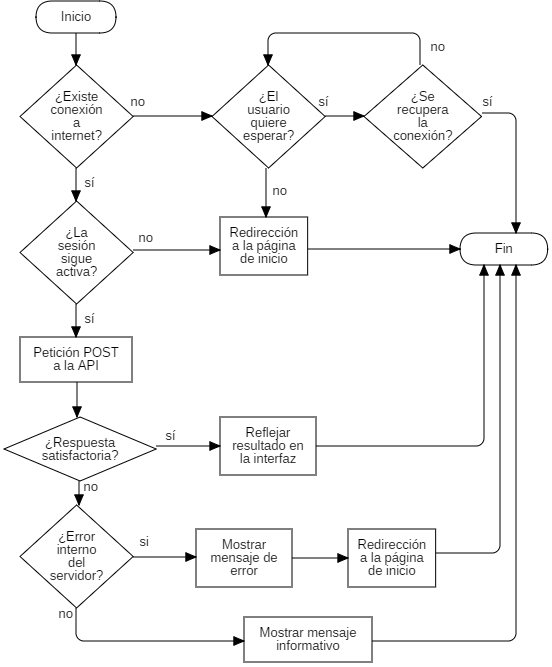
\includegraphics[width=1\textwidth]{../img/flowchart.png}
	\caption{Diagrama de flujo, peticiones POST a la API.}
	\label{fig:flowchart}
\end{figure}

Además, se tomó la decisión de que cada petición a la API, tanto POST como mediante WebSockets para la recepción de mensajes en tiempo real, se gestione por un hilo independiente. De esta forma se pueden recibir y mostrar datos de varias camas al mismo tiempo de forma sencilla y transparente. 

\subsubsection{Comunicación en tiempo real con \textit{Socket.IO}}

Al emplear esta biblioteca en la API, también debe usarse en el cliente para que la comunicación en tiempo real sea efectiva. 

A rasgos generales la comunicación se realiza en dos pasos: 

\begin{enumerate}
	\item Se conecta un \textit{Socket} a la ruta genérica del servidor y se emite un evento <<\texttt{give\_me\_data}>>. 
	\item Se conecta otro \textit{Socket} a la ruta formada por por la concatenación de la ruta genérica y el namespace que identifica la cama que se desea escuchar. A través de este \textit{Socket} se recibirán los eventos <<\texttt{package}>> con los datos en tiempo real. 
\end{enumerate}

\subsection{Autenticación}

La autenticación se resuelve de una forma muy sencilla desde el servidor. La primera petición POST que se debe realizar es la de autenticación, que recibe un nombre de usuario y una contraseña. Si el usuario tiene permiso para acceder al sistema, recibe un \textit{token} que se guarda como variable de sesión. Todas las peticiones POST sucesivas recibirán como parámetro este \textit{token}. 

\subsection{Actualización de la interfaz en tiempo real}

Para la funcionalidad de visualización de camas, la aplicación va a recibir continuamente los datos captados por la cama en tiempo real, y queremos que la interfaz se actualice cada vez que llega un dato. 

Dado que es un hilo el que gestiona la recepción de datos en tiempo real, para que la interfaz de usuario se actualice cada vez que se recibe un dato necesitamos implementar un mecanismo que permita que el hilo se lo notifique. La solución más sencilla que puede venir a la mente es el uso de un patrón observador. 

\begin{figure}[H]
	\centering
	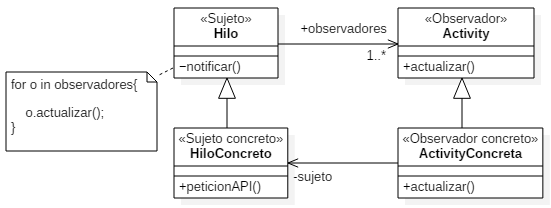
\includegraphics[width=1\textwidth]{../img/observador.png}
	\caption{Posible aplicación del patrón observador.}
	\label{fig:observador}
\end{figure}

Según se muestra en la figura~\ref{fig:observador}, la interfaz (Activity) tendría una referencia al hilo que realiza la petición, el que a su vez tendría una referencia a la interfaz. Desde su referencia a la interfaz, el hilo podría ejecutar el método \texttt{actualizar()}.

Esta es una solución muy simple y efectiva para muchas plataformas, pero no funciona en el caso de Android, ya que la actualización de los elementos de la interfaz (\textit{Layouts}) solo se puede realizar desde el hilo principal. Al llamar al método \texttt{actualizar()} desde el hilo, saltaría una excepción si dentro de este método se manipula algún elemento de la interfaz. 

Android ofrece varias alternativas para abordar este problema, y en mi caso he usado la que me ha parecido más sencilla: \textbf{el uso de \textit{Handlers}}~\cite{handler}. La idea es la misma, pero en este caso el \textit{Activity} tiene una referencia a un objeto \textit{Handler} que contiene el método \texttt{handleMessage}, el cual será el encargado de actualizar la interfaz. Cuando el \textit{Activity} lanza el hilo, le pasa la referencia al objeto \textit{Handler} como argumento. Cuando el hilo reciba un nuevo dato, se lo notificará ejecutando el método \texttt{sendMessage} del \textit{Handler}. Esta llamada activará el método \texttt{handleMessage} que, a diferencia del método \texttt{actualizar} del patrón observador, sí se ejecuta en el hilo principal. 

\subsection{Test de usabilidad}

De forma adicional a los test unitarios y los test de interfaz, se realizó un test de usabilidad tanto de la aplicación web generada por mi compañero José Luis Garrido Labrador como de mi aplicación Android. Este tipo de test involucra a los usuarios finales, y tiene como objetivo comprobar en qué medida el producto final cumple el propósito para el que fue diseñado y resulta adecuado y fácil de usar para los usuarios. 

Este test se realizó mediante una encuesta de Google~\cite{encuesta} que se difundió entre personas con perfiles sanitarios, educativos y tecnológicos principalmente. En esta encuesta se le proporcionaba un nombre de usuario y una contraseña al participante y se le pedía que realizara las siguientes tareas tanto en la aplicación web como en la aplicación Android: 

\begin{enumerate}
	\item Iniciar sesión con el usuario y contraseña que te hemos proporcionado. 
	\item Cambiar tu contraseña (ten en cuenta que una vez cambies tu contraseña deberás usar la nueva en cualquiera de las dos aplicaciones). 
	\item Consultar el estado de los pacientes. 
	\item Consultar las gráficas explicativas sobre el estado de los pacientes. 
	\item Cerrar sesión. 
\end{enumerate}

Para recoger las opiniones sobre cada una de las aplicaciones, se pedía al usuario que valorara las siguientes afirmaciones dos veces: una sobre la aplicación web y otra sobre la aplicación Android. Las valoraciones se daban entre 1 y 5 siendo 1=\textit{completamente en desacuerdo} y 5=\textit{completamente de acuerdo}. 

\begin{enumerate}
	\item Me ha resultado fácil realizar las tareas propuestas. (\textbf{Facilidad de uso})
	\item Me ha resultado fácil interpretar los elementos gráficos (iconos, botones, gráficas...). (\textbf{Interpretabilidad})
	\item La selección de elementos gráficos usados en la aplicación (colores, tipografías...) me ha parecido acertada. (\textbf{Uso de gráficos})
	\item La aplicación me ha parecido muy buena. (\textbf{Global})
\end{enumerate}

\subsubsection{Resultados del test}

En total, sobre las preguntas relativas a la aplicación Android respondieron 10 personas, cuyos perfiles profesionales se distribuyen como se muestra en la figura~\ref{fig:mobile_proportion}. 

En la figura~\ref{fig:mobile_general} se representa la valoración general de todos los usuarios en cada una de las afirmaciones. Como se puede ver, la valoración en general es muy positiva a excepción del caso de la interpretabilidad. Esto se puede deber a que en la encuesta se pide a los usuarios que realicen las tareas sin proporcionar demasiada información previa sobre la finalidad de la aplicación, más allá de que sirve para monitorizar el estado de pacientes con epilepsia mediante camas con sensores. Probablemente los usuarios finales de la aplicación necesitarían información adicional sobre qué representa cada gráfica y cómo interpretarlas. 

En la figura~\ref{fig:mobile_comparation} se comparan las valoraciones de los participantes con un perfil tecnológico con las de los participantes con un perfil no tecnológico (sanitario o educativo). Las valoraciones del perfil tecnológico son algo superiores que las del perfil no tecnológico, a excepción de la facilidad de uso de la aplicación, que es muy buena en los dos casos. 

\begin{figure}
	\centering
	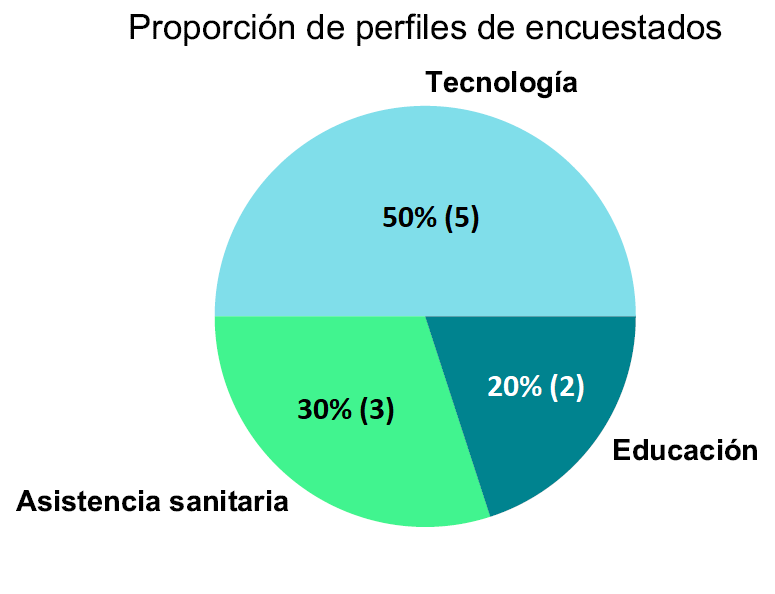
\includegraphics[width=0.7\textwidth]{../img/mobile_proportion.png}
	\caption{Proporción del perfil profesional de los participantes.}
	\label{fig:mobile_proportion}
\end{figure}

\begin{figure}
	\centering
	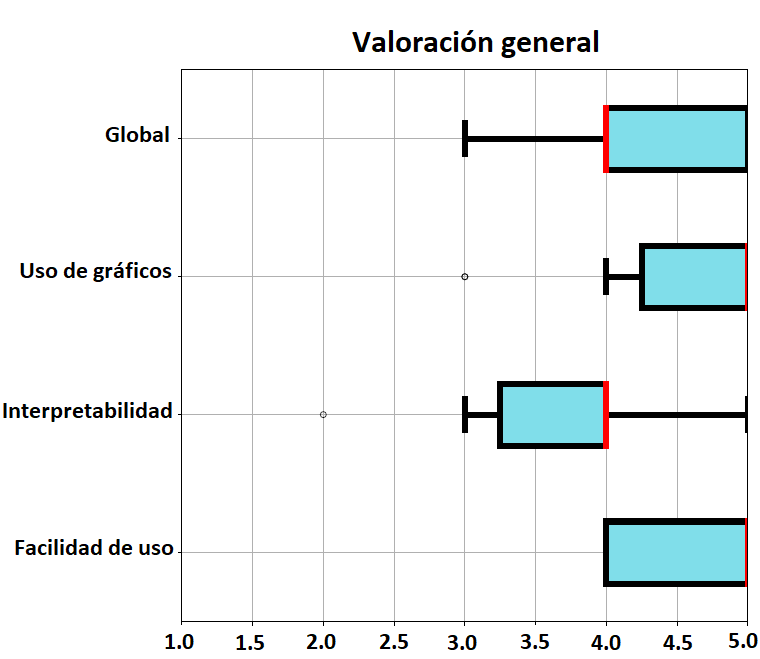
\includegraphics[width=0.7\textwidth]{../img/mobile_general.png}
	\caption[Valoraciones de todos los encuestados.]{Valoraciones de todos los encuestados. Los bigotes a izquierda y derecha de cada caja corresponden con los valores mínimo y máximo respectivamente. Los límites izquierdo y derecho de cada caja corresponden con el primer y tercer cuartil respectivamente. La línea roja corresponde con la mediana.}
	\label{fig:mobile_general}
\end{figure}

\begin{figure}
	\centering
	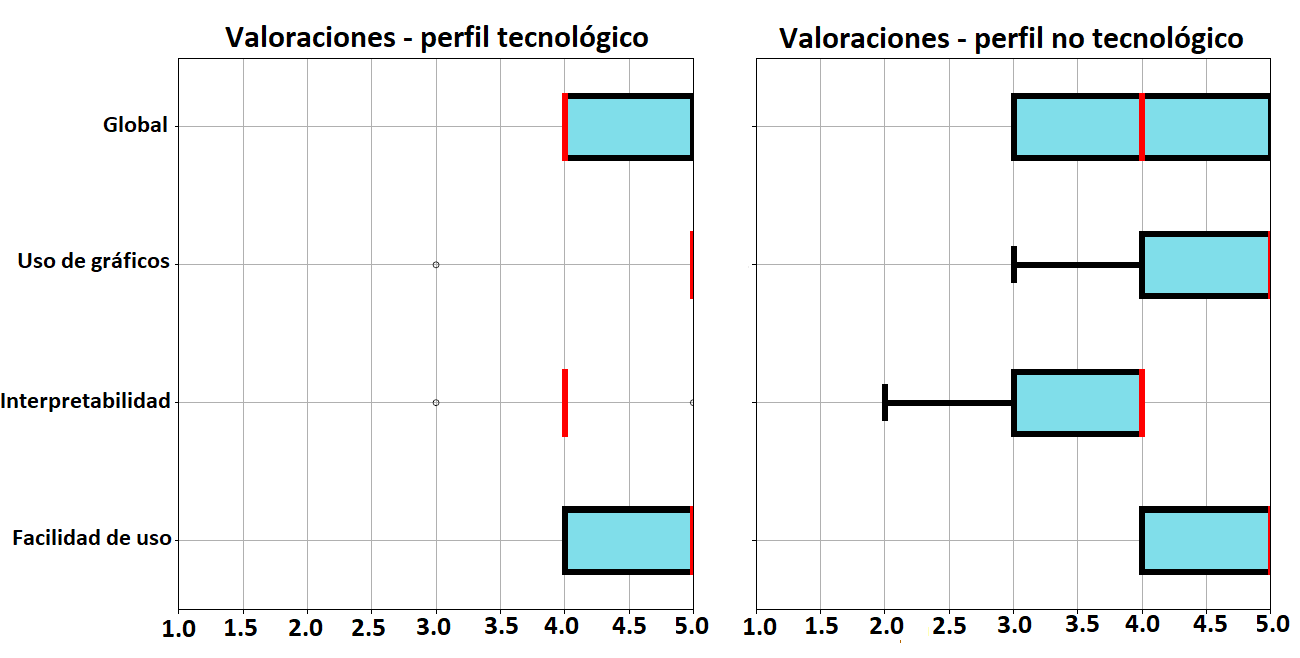
\includegraphics[width=1\textwidth]{../img/mobile_comparation.png}
	\caption[Comparación de valoraciones entre personas con perfil tecnológico y no tecnológico.]{Comparación de valoraciones entre personas con perfil tecnológico y no tecnológico. Los bigotes a izquierda y derecha de cada caja corresponden con los valores mínimo y máximo respectivamente. Los límites izquierdo y derecho de cada caja corresponden con el primer y tercer cuartil respectivamente. La línea roja corresponde con la mediana.}
	\label{fig:mobile_comparation}
\end{figure}

\section{Aspectos relevantes generales}

Este proyecto se me asignó gracias a la concesión de la \textbf{beca de colaboración de estudiantes en departamentos universitarios} del Ministerio de Educación, en este caso en el departamento de Ingeniería Civil. Esta beca tiene como objetivo la implicación del estudiante en un proyecto de investigación, ofreciendo la posibilidad de ampliar sus conocimiento y concretar sus intereses para la posible incorporación a futuras tareas docentes o investigadoras. 

La realización de este proyecto me ha permitido experimentar a grandes rasgos en qué consiste la labor de un investigador, y la experiencia, definitivamente, me ha llevado a considerar muy positivamente esta salida laboral. 

Otro aspecto relevante a señalar es que para la realización de este proyecto he trabajado junto con José Luis Garrido Labrador, de forma que muchas de las decisiones y las formas de trabajo se han decidido de forma conjunta, y en muchas partes del trabajo individual de cada uno se ha dependido en mayor o menor medida del trabajo del otro. Por un lado, su trabajo de investigación, relativo a la búsqueda del mejor \textit{ensemble} para la clasificación, se ha basado en mi extracción, filtrado y selección de características de series temporales, finalmente, mediante un algoritmo genético. Por otro lado, el desarrollo de mi aplicación Android depende directamente de la API del servidor remoto desarrollada por mi compañero. En este sentido, se puede considerar que este proyecto nos ha proporcionado cierta experiencia sobre el trabajo en equipo que se lleva a cabo en el día a día de una empresa real. 


